%header and footer for separate chapter files

\ifx\whole\undefined
\documentclass[12pt, leqno]{book}
\usepackage{graphicx}
\input style-for-curves.sty
\usepackage{hyperref}
\usepackage{showkeys} %This shows the labels.
%\usepackage{SLAG,msribib,local}
%\usepackage{amsmath,amscd,amsthm,amssymb,amsxtra,latexsym,epsfig,epic,graphics}
%\usepackage[matrix,arrow,curve]{xy}
%\usepackage{graphicx}
%\usepackage{diagrams}
%
%%\usepackage{amsrefs}
%%%%%%%%%%%%%%%%%%%%%%%%%%%%%%%%%%%%%%%%%%
%%\textwidth16cm
%%\textheight20cm
%%\topmargin-2cm
%\oddsidemargin.8cm
%\evensidemargin1cm
%
%%%%%%Definitions
%\input preamble.tex
%\input style-for-curves.sty
%\def\TU{{\bf U}}
%\def\AA{{\mathbb A}}
%\def\BB{{\mathbb B}}
%\def\CC{{\mathbb C}}
%\def\QQ{{\mathbb Q}}
%\def\RR{{\mathbb R}}
%\def\facet{{\bf facet}}
%\def\image{{\rm image}}
%\def\cE{{\cal E}}
%\def\cF{{\cal F}}
%\def\cG{{\cal G}}
%\def\cH{{\cal H}}
%\def\cHom{{{\cal H}om}}
%\def\h{{\rm h}}
% \def\bs{{Boij-S\"oderberg{} }}
%
%\makeatletter
%\def\Ddots{\mathinner{\mkern1mu\raise\p@
%\vbox{\kern7\p@\hbox{.}}\mkern2mu
%\raise4\p@\hbox{.}\mkern2mu\raise7\p@\hbox{.}\mkern1mu}}
%\makeatother

%%
%\pagestyle{myheadings}

%\input style-for-curves.tex
%\documentclass{cambridge7A}
%\usepackage{hatcher_revised} 
%\usepackage{3264}
   
\errorcontextlines=1000
%\usepackage{makeidx}
\let\see\relax
\usepackage{makeidx}
\makeindex
% \index{word} in the doc; \index{variety!algebraic} gives variety, algebraic
% PUT a % after each \index{***}

\overfullrule=5pt
\catcode`\@\active
\def@{\mskip1.5mu} %produce a small space in math with an @

\title{Personalities of Curves}
\author{\copyright David Eisenbud and Joe Harris}
%%\includeonly{%
%0-intro,01-ChowRingDogma,02-FirstExamples,03-Grassmannians,04-GeneralGrassmannians
%,05-VectorBundlesAndChernClasses,06-LinesOnHypersurfaces,07-SingularElementsOfLinearSeries,
%08-ParameterSpaces,
%bib
%}

\date{\today}
%%\date{}
%\title{Curves}
%%{\normalsize ***Preliminary Version***}} 
%\author{David Eisenbud and Joe Harris }
%
%\begin{document}

\begin{document}
\maketitle

\pagenumbering{roman}
\setcounter{page}{5}
%\begin{5}
%\end{5}
\pagenumbering{arabic}
\tableofcontents
\fi


\chapter{Fine moduli spaces}
\label{Moduli chapter}
\label{ModuliChapter}

\section{What is a moduli problem?}

Algebraic geometry is special among geometric theories in
that
the objects involved\emdash varieties,  schemes or maps between
them\emdash can be parametrized by other varieties or schemes. The set
of submanifolds of a given manifold, or more generally of maps between
two given manifolds, seems too large to be given the structure of a
finite-dimensional manifold itself. By contrast, any algebraic variety
is specified by a finite collection of polynomials, which in turn have
a finite number of coefficients, so it's not too far-fetched that the
set of all varieties with specified numerical invariants, or
morphisms between two given varieties, could be given the structure of
a ``moduli space'' that is a variety (or scheme or\dots) in its own
right.

For an example\emdash perhaps the original one\emdash projective plane
curves of degree $d$
are in natural one-to-one correspondence with the forms of degree $d$
modulo the group of nonzero scalars\emdash that is, with the points of
the dual of the projective space
$ \PP(H^0(\sO_{\PP^2}(d)))=\PP^{\sbinom{d+2}{2}-1} $.
Thus, for example, plane cubics are parametrized by $\PP^{9}$, and a
family $\cC \to B$ of cubics corresponds to a map $\phi: B \to \PP^9$ 
(Figure~\ref{cubic family}).
In this chapter, we'll give a general framework for the notion of moduli
space, introducing the main examples that we will treat in this book.

\begin{figure}
\vskip-14pt
$
  \vcenter{\hbox{\includegraphics[width=0.84in,trim=0 27 7 25,clip]{"main/Fig06-1a"}}}\hskip0.6em
  \vcenter{\hbox{\includegraphics[width=0.7in]{"main/Fig06-1b"}}}\quad
  \vcenter{\hbox{\includegraphics[width=0.7in]{"main/Fig06-1c"}}}\quad
  \vcenter{\hbox{\includegraphics[width=0.7in]{"main/Fig06-1d"}}}
$
\vskip-3pt
 \caption{A one-parameter family of plane cubics.}
 \label{cubic family}
\end{figure}

There are several ways in which the possibility of making moduli spaces
has been useful in algebraic geometry. First, the existence of a moduli
space that  parametrizes objects of a certain type allows us to speak
of the ``general \null object,'' meaning that we allow ourselves to avoid the
 properties of ``special objects'' parametrized by closed subvarieties
of the moduli space. For example, we can make precise sense of the
statement ``The general plane curve of degree $d$ is smooth.'' It means 
that the set of smooth curves corresponds to an open subset of the projective space $\PP^{\sbinom{d+2}{2}-1} $.
 We have already used this
possibility in many places in this book.

Second, it allows us to speak coherently about
families of objects. Some moduli spaces carry \emph{universal families},
\index{universal family}%
and every nice family of the sort of objects
they parametrize is pulled back from this one by a unique map.

This idea was already exploited informally in the nineteenth century in
\index{historical context}%
\index{preservation of number}%
the guise of ``preservation of number,'' used to count configurations of
points or curves with a given property by specializing the
data, and we have also exploited this idea in
Chapter~\ref{JacobianChapter} to explain the count of odd and even
theta characteristics on a general curve by appealing to the existence
of a specialization to a hyperelliptic curve. In a related manner, we
have already seen how the fact that invertible sheaves of degree $d$
on a curve $C$ are parametrized by a $g$-dimensional variety allows us
to prove the $g+3$ theorem (Theorem~\ref{g+3 theorem}).

Third, to the extent that we can describe the intersection theory of a
moduli space, it opens up the possibility of doing
enumerative geometry
\index{enumerative geometry}%
on it to count solutions of geometric problems\emdash and in particular
to prove the existence of solutions. For example, knowing that the
\index{P@$\PP^3$!any 4 curves intersect a common line}%
parameter space for lines in $\PP^3$ is the Grassmannian $\GG(1,3)$,
\index{Grassmannian $\GG(1,3)$}%
a projective variety of dimension 4, and that the condition that the
set of lines meeting a given curve of degree $d$
is a divisor linearly equivalent to  $d$ times the hyperplane section
(Figure~\ref{Chow degree}), we can conclude  that there exists a line
in $\PP^3$ meeting any four given curves \cite[Section 3.4.1]{3264}. We
will use the same idea to prove the much deeper existence of certain
linear series on all curves (the existence half of the Brill--Noether
theorem, discussed in Chapter~\ref{Brill--Noether}).

\begin{figure}
\centerline {\includegraphics[height=1.4in]{"main/Fig06-2"}}
 \caption{A general  one-parameter linear family of lines in $\PP^3$\emdash that is, the family of lines
 contained in a general plane and passing through a general point in that plane\emdash meets a space curve $C$ in
 $\deg C$ points.}
 \label{Chow degree}
\end{figure}

In modern terms, a \emph{moduli problem}
\index{moduli problem}%
consists of a class of objects
in algebraic geometry\emdash schemes, subschemes of a given scheme,
maps of schemes,
sheaves on schemes, typically defined by some common
attributes\emdash and a notion of what it means to have a \emph{family}
\index{family}%
of these objects parametrized by a scheme $B$. The notion is formalized
in the idea of a \emph{moduli functor},
\index{moduli functor}%
which associates to each scheme $B$ the set of families over $B$ of the
given sort. Examples will make this vague notion more concrete.

%\subsection*{Some moduli problems}

%\begin{enumerate}
%\label{list of moduli problems}

\begin{example}[effective divisors on a given curve] The objects are
\index{moduli functor}%
\index{effective divisor!family of --s on a curve}%
effective divisors of given degree on a given smooth, projective curve
$C$. A family of such divisors is a subscheme $\cD \subset B \times C$,
flat of degree $d$ over $B$.
Here we are using
the equivalence between divisors of degree $d$ on a smooth curve and
degree $d$ subschemes of the curve. The moduli space is the $d$-th
symmetric power
\index{symmetric power}%
$C_d$ of $C$, discussed in Section~\ref{symmetric section}.
\end{example}

\begin{example}[invertible sheaves on a given curve] The objects are
\index{invertible sheaves!family of --s on a curve}%
invertible sheaves on a given smooth projective curve $C$. A family
over a scheme $B$ is an equivalence class of invertible sheaves $\cL$
on $B \times C$ whose restriction to each fiber of $B \times C$ over
$B$ has degree $d$, where two families $\cL$ and $\cL'$ on $B \times
C$ are equivalent if $\cL\cong \cL' \otimes \cM$, where $\cM$ is  an
invertible sheaf pulled back from $B$. Usually one restricts attention
to invertible sheaves
whose restrictions to each fiber $b\times C$ have a given degree $d$.
\index{Jacobian}%
\index{Picard variety}%
The moduli spaces are the Jacobian and Picard varieties,
discussed in
Section~\ref{Picard section}.
\end{example}

\begin{example}[moduli of smooth curves] The objects are isomorphism
\index{smooth curve!moduli of --s}%
classes of smooth, projective curves of genus $g$. A family over $B$
is an equivalence class of smooth, projective morphisms $f : \cC \to B$
whose fibers are curves of genus $g$, where two such families $f, f'$
are equivalent if there is an isomorphism from the source of $f$ to
the source
of $f'$ making the
following diagram commute:
$$
\begin{diagram}[small]
\cC && \rTo^\cong && \cC'\\
&\rdTo_f&&\ldTo_{f'}\\
&&B
\end{diagram}
\vspace*{3pt}
$$
The moduli spaces $M_g$ of curves are harder to construct, and we will
have a separate discussion of them in
Chapter~\ref{CurvesModuliChapter}. Nonetheless,
it will be useful at several points in this chapter to assume their
existence.
\end{example}

\begin{example}[Hurwitz spaces] An object is a smooth projective curve $C$
\index{Hurwitz space}%
of a given genus, together with a map $f: C\to \PP^1$ of given degree, up
to isomorphisms of the curves that commute with the map, as in this diagram:
$$
\begin{diagram}[small]
C && \rTo^{\cong} && C'\\
&\rdTo_f&&\ldTo_{f'}\\
&&\PP^{1}
\end{diagram}
$$
A family over $B$ is a family $\cC \to B$ of smooth projective curves
of a given genus, together with flat map $\cC \to B\times \PP^{1}$
of degree $d$.
 Often the allowable ramification indices are specified. We will discuss
 the simplest Hurwitz scheme in Chapter~\ref{CurvesModuliChapter}.
\end{example}

\begin{example}[Severi varieties] The objects are plane curves
\index{Severi variety}%
\label{Severi}%
of given degree $d$ and geometric genus $g$. If $g \neq \tbinom{d-1}{ 2}$
the curves will necessarily be singular, but are often
constrained to have only mild singularities, usually only nodes. We will
discuss
Severi varieties
in Chapter~\ref{CurvesModuliChapter}.
\end{example}

\begin{example}[Hilbert schemes] The objects are subschemes of a given
\index{Hilbert scheme}%
projective space;   a family over $B$ is a subscheme $\cC \subset B \times
\PP^r` `$, flat over $B$. Since the Hilbert polynomials of the fibers
of a
flat family
\index{flat family}%
are all equal
\cite[Chapter III, \S9]{Hartshorne1977},
the Hilbert scheme is the disjoint union of subschemes corresponding to
particular Hilbert polynomials, and these subschemes are of finite type.
\index{finite type}%
If $B$ is reduced then the flatness condition is equivalent to the
constancy of the Hilbert polynomial (\cite[Theorem 9.9]{Hartshorne1977} or \cite[Chapter III, \S 3.2]{DE-JH-schemes}).

In Chapter~\ref{HilbertSchemesChapter} we
study the
open set consisting of smooth curves $C\subset \PP^{r}$ of given degree
and genus.
\end{example}

\section{What is a solution to a moduli problem?}

Typically what we want from a solution to a
moduli problem
\index{moduli problem}%
is to
understand all possible families of the objects
in question. In particular, the individual objects should be in natural
\index{natural correspondence}%
one-to-one correspondence with the closed points of the
moduli space.  The word \emph{natural} is the key. Most of the time,
the set of objects we are interested in has
the cardinality of the continuum,
as do all positive-dimensional varieties $M$ over $\CC$, so a mere
bijection between the points of $M$ and the objects to be parametrized
is meaningless.

In the nicest situations there is a
\emph{universal} family
\index{universal family}%
$\phi:
\cX\to M$ of these objects over $M$,
such that any family over a scheme $B$  is pulled back from the one on
$M$ via a unique morphism $B\to M.$  Such a space $M$ with its universal
family $\phi$, if it exists, is called a \emph{fine moduli space}. This
\index{fine moduli space}%
\index{moduli space!fine}%
can be expressed more abstractly but more succinctly by saying that the
moduli scheme \emph{represents the moduli functor}, which means there
is an isomorphism of functors
$$
\{ B \mapsto \text{families of } X \text{ over } B \} \cong \{ B\mapsto
\mathrm{{Mor}}_{\mathrm{ Schemes}}(B, M) \}.
$$
If $M$ is a fine moduli space then the identity map $M\to M$ corresponds
to the ``universal family'' $\phi: \cX \to M$.
The Hilbert scheme, as well as $\Div_d(C)$ and $\Pic_d(C)$ are fine moduli
spaces but the moduli space of curves
and the Hurwitz schemes are not.

If a fine moduli space and its universal family exist, then it is unique
up to unique isomorphism: given two avatars $M$ and $M'$
the universal family on $M$ corresponds to a map $M\to M'$, and we
similarly produce a map $M'\to M$. The pullback of the universal family
on $M$ by the composition of these two maps is again the universal family,
so the composition is the identity map.

Although the moduli space of curves and the Hurwitz spaces are not fine
moduli spaces, they are still defined
in a way that makes them unique, as we shall see below.

\def\eps{{\epsilon}}
One of the useful features of a fine moduli space is that it makes the
computation of tangent spaces relatively easy.
\index{tangent space}%
\index{Zariski tangent space}%
Recall that if $(R,\gm)$ is the local ring at a point $m$ on a variety
$\cM$ then the (Zariski) tangent
space to $M$ at $m$ is the vector space of linear functionals
$\Hom_{R/\gm}(\gm/\gm^2, R/\gm)$.   Assuming that
$R$ contains its residue field $k \colonequals  R/\gm$, such functionals
are precisely the restrictions to $\gm/\gm^2$ of the ring homomorphisms
$R \to k[\eps]/(\eps^2)$ inducing the identity on $k$.
 If $\cM$ is a fine moduli space for some functor $F$, then such maps
 are in one-to-one correspondence
with the set $F(E)$ of families over $E \colonequals
\Spec(k[\eps]/(\eps^2))$.

The vector space structure on the tangent space is also accessible from
this description:  the
 sum of tangent vectors corresponding to families $X_i \to E$ is the
 restriction to the diagonal
 $E \subset E\times E$
 of the product family $X_1 \times X_2 \to E\times E$.
Often one can to compute the tangent space to a moduli space before even
knowing that the moduli space exists!

\section{Hilbert schemes}
\label{hilbert scheme section}

The Hilbert scheme is a fine moduli space representing the functor of
\index{flat family!of subschemes}%
\index{subscheme!family of --s}%
\index{Hilbert scheme|(}%
flat families of subschemes of $\PP^r` `$,
that is, the functor that takes a scheme $B$ over $\CC$ to the set of
subschemes $\sX \subset B\times \PP^r$
that are flat over $B$; a morphism $f: B'\to B$ induces a map carrying
a family to the pullback of the family by $f$.

\begin{example}[the Hilbert scheme of plane curves]
\label{Hilb for plane curves}
Let $p(m) \colonequals  dm+1-\tbinom{d-1}{ 2}$ be the Hilbert polynomial of
a
plane curve
\index{plane curve}%
of degree $d$, and consider the family
$\Hilb_{p(m)}(\PP^2)$
\index{notation!$\Hilb_{p(m)}$}%
of schemes $X \subset \PP^{2}$ having Hilbert polynomial $p$. Since
$\dim X = \deg p = 1$, $X$ has at least one component that is
1-dimensional. The union of such components must have degree
equal to $d$, the leading coefficient of $p(m)$. Since the Hilbert
polynomial  of this union is also equal
to $p(m)$ we see that $X$ is in fact a (possibly nonreduced and/or
reducible) plane curve of degree $d$. The space $\Hilb_{p(m)}(\PP^2)$
is the projective space $\PP^{\sbinom{d+2}{2}-1}$ of forms of degree $d$,
and the universal family is the projection
universal family
\index{universal family}%
$$
\bigl\{@(x,F) \in \PP^2 \times \PP^{\sbinom{d+2}{2}-1} \mid F(x)=0@\bigr\} \to
\PP^{\sbinom{d+2}{2}-1}.
$$

More typically, the set of curves $C \subset \PP^r$ of degree $d$ and
genus $g$ corresponds to a subset of the Hilbert scheme parametrizing
subschemes of $\PP^r$ with Hilbert polynomial $p(m) = dm - g + 1$, though
not all schemes with this Hilbert polynomial are purely one-dimensional
subschemes, as we shall see.
\end{example}

In this section
we
compute
the Zariski tangent space to the Hilbert scheme at a point and
\index{Zariski tangent space}%
\index{Hilbert scheme!at a point}%
sketch the construction of the scheme itself. For a rigorous
treatment including many generalizations,  see \cite{HomogHilbert}
or \cite{MR2222646}. In Chapter~\ref{HilbertSchemesChapter}, we'll
describe  the
open subsets of smooth curves in the Hilbert schemes of curves of low
degree and genus in $\PP^3$ in more detail.

\subsection[The tangent space to the Hilbert scheme]{\hskip-3pt The tangent space to the Hilbert scheme}
%\label{tan hilbert section}

Following the general recipe for tangent spaces to fine moduli spaces,
we need to understand
flat families
\index{flat family}%
of projective schemes over $E \colonequals  \Spec
\CC[\eps]/(\eps^2)$. Recall
from
\cite[p.\,182]{Hartshorne1977},
for example,
that if
$X\subset \PP^r$ is a smooth subscheme then
 the normal bundle $\sN_{X/\PP^r}$ of $X$ in $\PP^r$ is defined in terms
 of the tangent bundles
 of $X$ and $\PP^r$ by the exact sequence:
$$
0\to \sT_X \ruto {\phi} \sT_{\PP^r}|_X \to \sN_{X/\PP^r} \to 0.
$$
Thus a global section of
$\sN_{X/\PP^r}$
\index{infinitesimal motion of a curve}%
can be thought of as an infinitesimal motion of~$X$ (Figure~\ref{perturbed
curve}).

\begin{figure}
\centerline {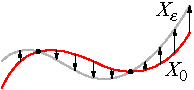
\includegraphics[width=1.35in]{main/Fig06-0-new}}
\vskip-5pt
 \caption{Infinitesimal perturbation of a curve by a normal vector field.}
 \label{perturbed curve}
\end{figure}

To define the normal sheaf for locally complete intersection subschemes
$X$ we first define the
\emph{conormal sheaf}
\index{conormal sheaf}%
to be the kernel of the dual  of $\phi$, which is the natural map
$\Omega_{\PP^r}|_X \to \Omega_X$,
and since $X$ is locally a complete intersection, this corresponds to
the exact sequence:
$$
0\to \sI_{X/\PP^r}/\sI_{X/\PP^r}^2 \to \Omega_{\PP^r}|_X \to \Omega_X
\to 0.
$$
We thus define $\sN_{X/\PP^r} \colonequals
\sHom(\sI_{X/\PP^r}/\sI_{X/\PP^r}^2, \sO_X)$.

By analogy we define the
\emph{normal sheaf} of any subscheme $X\subset
\index{normal sheaf}%
\PP^r$
$$
\sN_{X/\PP^r} \colonequals  \sHom(\sI_{X/\PP^r}/\sI_{X/\PP^r}^2, \sO_X).
$$
The following theorem shows that this
has the same connection with infinitesimal motions for arbitrary
subschemes $X$.

\begin{theorem}
\label{tangent space of Hilb}
Let $X\subset \PP^r$ be a subscheme with Hilbert polynomial $p(m)$ and let
$E = \Spec\CC[\eps]/(\eps)^{2}$. The flat families
$\sX \subset \PP^r\times E$ specializing to $X$ at the closed point
defined by $(\eps)$
are in natural one-to-one correspondence with the vector space
\index{Zariski tangent space!to the Hilbert scheme}%
$\Hom_{\PP^r}(\sI_{X/\PP^r}, \sO_X) = H^0(\sN_{X/\PP^r})$, which is thus
the tangent space to the Hilbert scheme $\Hilb_{p}(\PP^r)$ at $[X]$.
\end{theorem}

\begin{proof}
We will actually treat the analogous result for an affine subscheme $X
\subset \AA^r = \Spec S$, where
$S = \CC[x_{1}, \dots, x_{r}]$; since our construction is natural,
it will patch on an affine cover to give the projective case stated above.

An $E$-module $M$ is flat
\index{flat module}%
over $E$ if and only if $\Tor_1^E(\CC,M) = 0$.
Since the
free resolution
\index{free resolution}%
of $\CC$ as an $E$-module has the form
$$
\cdots \ruto {\ \eps} E \ruto {\ \eps} E \ruto {\ \eps} E
\ruto{}\ \ \CC \ruto{}\ \ 0,
$$
we have $\Tor_1^E(\CC,M)=0$ if and only if the submodule of $M$
annihilated by $\eps$ is $\eps M$.

We first construct a flat family from a homomorphism: Let
$$I = (g_1,\dots,
g_t)\subset S = \CC[x_1,\dots, x_r]
$$
be the ideal defining $X$.
Note that $\Hom_S(I/I^2, S/I) = \Hom_S(I,S/I)$. Let $\phi: I\to S/I$
be a homomorphism, and let $h_i\in S$ be
any element reducing to $\phi(g_i)$ modulo $I$.  The ideal
$$
I' \coloneqq  (g_1+\eps h_1,\dots, g_t+\eps h_t)\subset
S[\eps]/(\eps^2) \equalscolon S'
$$
defines a scheme $\Spec S'`/@I'$  over $E$ which restricts to $X$ modulo
$(\eps)$; that is, $I' +\nobreak (\eps) =\nobreak  I$.

To see that $I'$ is
independent of the lifting chosen,
consider
$k_1,\dots,k_t\in I$
such
that the elements $g_i+\eps(h_i+k_i)$ are a different lifting,
generating an ideal~$I''$.
Writing $k_i = \sum r_{i,j}g_j$ we have
$$
g_i+\eps(h_i+k_i) = g_i+\eps h_i+ \sum \eps r_{i,j}(g_j+\eps h_j)
,
$$
 so
$I'' \subset I'$, and symmetrically $I' \subset I''$.

To prove flatness, suppose that $a\in S'$ and  $\eps a  \in I'$,
so that we can write  $\eps a= \sum(r_i+\eps s_i)(g_i+\eps h_i)$ for
some $r_{i}, s_{i} \in S$.
It follows that
$\sum r_i\g_i = 0$. Since $\phi$ is a homomorphism this implies $\sum
r_i h_i \in I$. Thus
$\eps a \in  \eps I\subset S'$, whence $a\in I + (\eps)$.  Writing $a
=\sum p_i g_i+\eps b'$
and using the relations $g_i \equiv -\eps h_i \hbox{ mod } I'$ we get
 $a \equiv \eps (-\sum p_i h_i+b') \hbox{ mod } I'$, as required.

Finally, starting from a flat family $S'`/@I'$ over $E$ with $I' + (\eps)
= I +\eps$,
let $J$ be the image of $I'$ in $S'/(\eps I) = S \oplus (\eps S)/(\eps
I)$. We claim that $J$ is the graph of a homomorphism $\phi: I \to
(\eps S)/(\eps I) \cong S/I$.

Since $I' + \eps S = I +\eps S$,  the projection  to the  summand
$S\subset S'$ maps $J$ onto~$I$.
To prove that $J$ is the graph of a homomorphism, it suffices to show
that this projection is an isomorphism.
The kernel is
the intersection of $J$ with $(\eps S)/(\eps I )$, so we must show that
if $r\in S$ and $\eps r \in I'$ then $\eps r \in \eps I$.

Since $\eps r \in I'$, the condition of flatness implies
that the image of $r$ in $S'`/@I'$ is in $\eps(S'`/@I')$, which is to say
that $r \in I' + \eps S = I +\eps S$.
Thus $r \in  I + \eps S,$ whence $\eps  r \in \eps I$ as required.

This shows that
$J$ is the graph of a homomorphism $\phi$ such that
 $I'$ is generated by $\{g+\phi g\mid g\in I\}$, so the two constructions
 are inverse to
each other.
\end{proof}

\begin{example}
\label{Hilb for plane curves-continued}
If $C$ is the
plane curve
\index{plane curve!Hilbert scheme}%
of degree $d$ defined by a form $F$, then the
ideal sheaf of $C$ is $\sO_{\PP^2}(-d)$, and thus
$$
\sHom(\sI_{C/\PP^2}/\sI_{C/\PP^2}^2, \sO_{C}) = \sO_{\PP^2}(d)|_C =
\sO_C(d).
$$
From the exact sequence
$$
0\to\sO_{\PP^2}\ruto {\,F}\sO_{\PP^2}(d) \to\sO_C(d)\to 0
$$
we deduce that the dimension of the tangent space to
$\Hilb_{p(m)}(\PP^2)=\PP^{\sbinom{d+2}{2}-1}$  at $C$
with $p(m) = dm+1-\tbinom{d-1}{ 2}$,
is $h^0(\sO_C(d)) = h^0(\sO_{\PP^2}(d))-1 = \dim \PP^{\sbinom{d+2}{2}-1}$,
as expected.
\meshing
\end{example}

\subsection{Parametrizing twisted cubics}

By Lemma~\ref{smooth is open}
below, the set of twisted cubics\emdash that is, smooth, irreducible,
nondegenerate curves of degree 3 in $\PP^3$\emdash is an open subset
of the Hilbert scheme $\Hilb_{3m+1}(\PP^3)$. As we've seen, a twisted
\index{twisted cubic}%
cubic curve $C \subset \PP^3$ can be described as the zero locus of
three homogeneous quadratic polynomials $Q_1, Q_2$ and $Q_3$ in the
homogeneous coordinates on $\PP^3$; to specify the twisted cubic
we could just list the $3 \times 10 = 30$ coefficients of these. But
of course we could replace the three quadrics $Q_i$ with any three
independent linear combinations of them; what matters\emdash and what
is naturally associated to $C$\emdash is the vector space $V = \langle
Q_1, Q_2, Q_3 \rangle \subset H^0(\cO_{\PP^3}(2))$. This suggests that
we consider the map of sets
$$
h : \{ \text{twisted cubic curves } C \subset \PP^3 \} \to G = G(3,
H^0(\cO_{\PP^3}(2)))
$$
obtained by associating to a twisted cubic $C$ the second graded piece
of its homogeneous ideal.

This differs significantly from
the example of plane curves introduced in the second paragraph of this chapter (page~\pageref{ModuliChapter}; see also Examples \ref{Hilb for plane curves} and \ref{Hilb for plane curves-continued}):
there, the objects to be parametrized were the
zero locus of a single polynomial, and we could vary those coefficients
arbitrarily and still have a plane curve; thus, the image of the analogous
map was open in the projective space $\PP^{\sbinom{d+2}{2}-1}$. But if
we generically
perturb the coefficients of the three quadratic polynomials $Q_i$
defining the twisted cubic the resulting quadrics will
be a complete intersection, generating
 the ideal of a set of eight points. Thus the image of the map $h$
 does not contain an open set of $G$.
We will give equations defining the image in Section~\ref{hilb
construction}, and we can consider it
the Hilbert scheme of twisted cubics.

As in this case, we will mainly be   interested in the subsets of the
Hilbert schemes corresponding to smooth irreducible curves:

\begin{lemma}
\label{smooth is open}
Suppose that $X \to B$ is a flat family of projective schemes (that is,
\index{flat family of projective schemes}%
the projection to the second factor of
$X\subset B\times \PP^n$  is flat). The points $b\in B$ such that the
fiber $X_b$ is smooth and irreducible form an open set.
\end{lemma}

\begin{proof}
To prove the
lemma we may assume that $B = \Spec A$ is affine and
irreducible. Let $x_{0}\dots, x_{r}$ be homogeneous coordinates
on $\PP^{r}$, and suppose that
$X\subset \PP^{r}_{\CC}$ is defined by the ideal $I_{X} = (F_{1}, \dots,
F_{n}) \in A[x_{0}, \dots x_{r}]$.
Since $X$ is flat over $B$ the fiber dimension $d$ is constant, and the
singular locus
of a given fiber $X_{b}$ is  the subscheme of $X_{b}$ defined by the
ideal $J$ of
$(r-d)\times (r-d)$ minors of the Jacobian matrix $(\partial
F_{i}/\partial x_{j})$.

Let $Y\subset B\times \PP^{r}$ be the closed subscheme defined by $J$
alone.
It follows that $Y\cap X \subset X$ defines a scheme of singular points
of fibers of the family, so this set is closed
in $X$.
Since the map $X \to B$ is projective, the image of $X\cap Y$ is closed,
and its complement is open.
 Finally, a smooth fiber $X_b$ is irreducible if and only~if it is
 connected. This holds if and only if $h^0(\sO_{X_b}) <2$ and by the
base change theorem
\index{base change theorem}%
\cite[Theorem 12.11]{Hartshorne1977} this set
 is open as well.
\end{proof}

\begin{proposition}
\label{hilb of twisted cubics}
The open subset $\cH^\circ$ of the Hilbert scheme $\Hilb_{3m+1}(\PP^3)$
para\-metrizing twisted cubics is irreducible of dimension $12$.
\unif
\end{proposition}

\begin{proof}
Let $C_0 \subset \PP^3$ be a twisted cubic, and consider the family
\index{PGL@$\PGL_4$}%
of translates of $C_0$ by automorphisms $A \in
\PGL_4
$ of $\PP^3$:
that is, the family
$$
\cC = \bigl\{@(A, p) \in \PGL_4 \times \PP^3 \; \mid \; p \in A(C_0)@\bigr\}.
$$
Via the projection $\pi : \cC \to \PGL_4$, this is a family of twisted
cubics, and so it induces a map
$$
\phi : \PGL_4 \to \cH^\circ.
$$
Since every twisted cubic is a translate of $C_0$, this is surjective,
with fibers isomorphic to the stabilizer of $C_0$, that is, the subgroup
of $\PGL_4$ of automorphisms of $\PP^3$ carrying $C_0$ to itself. By
Exercise~\ref{projective automorphism}, every automorphism of $C_{0}$ is
induced by an automorphism of $\PP^{3}$, so the stabilizer is isomorphic
to $\PGL_2$ and  thus has dimension 3. Since $\PGL_4$ is irreducible of
dimension 15, we conclude that $\cH^\circ$ is irreducible of dimension 12.
\end{proof}

\subsection{Construction of the Hilbert scheme in general}
\label{hilb construction}

The Hilbert scheme is more complicated than would appear from the examples
above, and this is even true
for the Hilbert polynomial $3m+1$. There are many subschemes of $\PP^3$
that have the same Hilbert polynomial $3m+1$ as a twisted cubic\emdash
for example, the union of a plane cubic and a point\emdash and are
not the intersection of the quadrics containing them. (See Exercises
\ref{characterization of degree} and~\ref{deg of disjoint union}.) In
Chapter~\ref{HilbertSchemesChapter} we will discuss many more components
of Hilbert schemes.

A fundamental result of
\index{Matsusaka, Teruhisa}%
Matsusaka provides a place to start:

\begin{npt}
\begin{theorem}[\cite{Matsusaka}]
\label{matsusaka}
Let $p(m) \in \QQ[m]$ be a polynomial. There exists an integer $m_0$
\index{Matsusaka's theorem}%
such that:

\begin{enumerate}
\item For any subscheme $X \subset \PP^r$ with Hilbert polynomial
$p_X = p$ we have
$$
h^0(\cI_{X/\PP^r}(m)) = \mbinom{m+r}{r} - p(m) \quad \text{for all }
m \geq m_0;
$$
in other words, the Hilbert function of $X$ agrees with the Hilbert
polynomial $p_X = p$ for all $m \geq m_0$.

\item For any subscheme $X \subset \PP^r$ with Hilbert polynomial $p_X =
p$ and
the saturated ideal of $X$ is defined by forms of degree $\leq m$.
\end{enumerate}
\end{theorem}
\end{npt}

Note that for any given $X$ the existence of an $m_0$ satisfying the
\index{Serre--Grothendieck vanishing theorem}%
statement of the lemma is immediate by
Theorem~\ref{Serre--Grothendieck vanishing}. The point of the lemma is
that we can find one value of $m_0$ that works for all $X$ with
Hilbert polynomial $p$. The following result of Gotzmann~\citeyear{Gotzmann}
provides a method for determining $m_0$.

\begin{theorem}
The Hilbert polynomial  of the homogeneous coordinate ring of any scheme
$X\subset \PP^r$ can be written uniquely in the form
$$
\chi(\sO_X(m)) = \mbinom{m+a_1}{a_1}+ \mbinom{m+a_2 -1}{a_2}+ \cdots+\mbinom{m+a_s -(s-1)}{a_s}
$$
with
$$
a_1\geq \cdots \geq a_s \geq 0,
$$
where the binomial coefficients are interpreted as polynomials in
$m$. Moreover, the saturated homogeneous ideal of $X$ is
 generated in degrees $\leq s$, and one can take $m_0 = s$ in the
 construction of the Hilbert scheme above.
\unif
\end{theorem}

See \cite{MR1023391} %Green-Gotzmann
for an exposition and a proof. From the coefficients $a_j$ one can read
off uniform vanishing theorems for $H^i(\sI_X(m))$
 as well.

 For example, the Hilbert polynomial $3m+1$ of the twisted cubic may be
 written as
 $$
 3m+1 =  \mbinom{m+1}{1}+ \mbinom{m+1 -1}{1}+\mbinom{m+1 -2}{1}+
\mbinom{m+0 -3}{0},
 $$
 Here $s=4$, and indeed the homogeneous ideal of the union of a plane
 cubic with a point, also in the plane,
 requires equations of degree 4.

\subsection{Grassmannians}
\label{Grassmannian section}

The
simplest and most fundamental
Hilbert schemes are the
Grassmannians\emdash including the projective spaces themselves.
\index{Grassmannian}%
They
\null
parametrize the families of linear subspaces of given dimension in
vector spaces or in projective spaces.
For $0\leq k\leq r$ we write $\GG(k,r)$ for the set of $k$-planes in
\index{notation!$\GG(k,r)$}%
$\PP^{r}$ and identify it with
$G(k+1,r+1)$, the set of $(k+1)$-dimensional vector subspaces of an
$(r+1)$-dimensional vector space.
When we want to make the $(r+1)$-dimensional vector space $V$ explicit,
we write $G(k+1, V)$ instead.

We embed $G(k+1,V)$ in $\PP\bigl(\mwedge^{r-k}V\bigr)
= \PP^{\sbinom{r+1}{r-k}-1}$
by sending a subspace $W\subset V$ to the 1-quotient $\mwedge
\vbox to 7.5pt{}^{r-k}V \to
\mwedge\vbox to 7.5pt{}^{r-k}(V/W)$.
This map is a monomorphism called the \emph{Pl\"ucker
\index{Pl\"ucker embedding}%
embedding}, and its image is an algebraic subvariety, which we take to
be the algebraic structure
of the Grassmannian.
{\meshing[-3pt]\par}

Concretely,
choose a basis of $V/W$ so that the projection map $V \to V/W$ is
given by an $(r-k)\times (r+1)$
matrix $A$. The coordinates of the image of $W$ are the $(r-k)\times
(r-k)$ minors of $A$,
called \emph{Pl\"ucker coordinates} of $W` `$. On the open set where
\index{Pl\"ucker coordinates}%
the first $(r-k)\times (r-k)$
minor is nonzero, we may multiply by its inverse, and it is not hard to
check that the
minors become the entries of the complementary $k \times (r-k)$
submatrix; thus
 $G(k,V)$ is covered by open sets isomorphic to affine $k(r-k)$-space,
so that
$G(k+1,r+1) = \GG(k,r)$ is smooth and
 irreducible of dimension $k(r-k)$.

\begin{example}
The Grassmannian $\GG(1,3)$ of lines in $\PP^{3}$ has Pl\"ucker
coordinates of a line
$L$ that is the span of points $q,r\in \PP^{3}$ the $2\times 2$ minors
of the $2\times 4$ matrix
whose rows are the coordinates of the points:
$$
\begin{pmatrix}
q_{0}&q_{1}&q_{2}&q_{3}\\
r_{0}&r_{1}&r_{2}&r_{3}\\
\end{pmatrix}
.
$$
Indexing the minors $p_{i,j}$ by pairs of distinct column indices one
can easily prove the
\emph{Pl\"ucker relation}
\index{Pl\"ucker relation}%
$$
p_{0,1}p_{2,3} - p_{0,2}p_{1,3}+p_{0,3}p_{1,2} = 0,
$$
and this defines $\GG(1,3)\subset \PP^{5}$ as a quadric hypersurface.
\end{example}

\def\sW{{\mathcal W}}

The \emph{universal subbundle} $\sW \subset V\times G(k+1,r+1)$, also
\index{universal subbundle}%
\index{tautological subbundle}%
called the \emph{tautological subbundle},  is
the vector bundle with fiber
 $W\subset V$ over the point of $G(k+1,V)$ corresponding to $W` `$. It
 is universal in the sense that
 given any scheme $X$ and a $(k+1)$-dimensional subbundle $\sW'$ of
 the trivial bundle $V\times X$
there is a unique morphism $X\to G(k+1,V)$ such that the pullback of $\sW$
is $\sW'$.

For a thorough introduction to the Grassmannian,
%(
the reader may consult
Chapters 3--4 of
\cite{3264}.

\subsection{Equations defining the Hilbert scheme}
\label{eqns of Hilb}

Matsusaka's theorem allows us to define an injective map of sets
\index{Matsusaka's theorem}%
$$
h : \left\{ \text{subschemes $X \subset \PP^r$ with $p_X=p$} \right\}
\to G\left(\tbinom{m_0+r}{r} - p(m_0),\tbinom{m_0+r}{r} \right)
$$
by sending $X$ to $H^0(\cI_{X/\PP^r}(m_0))$, and its image is the set
of closed points of the Hilbert scheme.
It remains to describe the scheme structure.

We observed above that though there are vector spaces $V$ of 3 quadrics
in $\PP^{3}$ that define
twisted cubics, a general such vector space  would generate the ideal of
8 points,  not a twisted cubic. What we want to know is how to tell
these cases apart algebraically. Consider the multiplication map
$$
V \otimes H^0(\cO_{\PP^3}(1)) \to H^0(\cO_{\PP^3}(3)).
$$
We saw in Chapter~\ref{genus 0 and 1 chapter} that the cokernel of this
map is the 10-dimensional space $H^0(\sO_{\PP^1}(9))$, so the image of
this map is 10-dimensional, whereas
3 general quadrics form a complete intersection and would have only
Koszul syzygies, so
in the case of general quadrics this map would have 12-dimensional image.
This is a map from a 12-dimensional vector space to a 20-dimensional one,
and what we've seen is that if $V$ is the net of quadrics containing a
twisted cubic, it~has a 2-dimensional kernel; that is, it has rank 10.

Thus if $\cE$ is the universal subbundle on
$$G = G(3, H^0(\cO_{\PP^3}(2))),$$
and  $H^0(\cO_{\PP^3}(d))\otimes \sO_G$ is the
trivial bundle, then the multiplication map above gives a map of vector
bundles
$$
\mu: \cE \otimes H^0(\cO_{\PP^3}(1)) \to H^0(\cO_{\PP^3}(3)).
$$
We can represent this locally as a matrix of functions, and the $11\times
11$ minors of this matrix
define the rank 10 locus, and thus vanish on the points of
the Hilbert scheme: in a neighborhood of a point in $G$ corresponding
to a twisted cubic, the common zero locus of these minors is the locus
of nets of quadrics containing a twisted cubic.

In fact, the construction of the Hilbert scheme in general is no more
structurally complicated than this special case. Given a polynomial
$p(m)$, we find a value of $m_0$ that satisfies the statement of
Theorem~\ref{matsusaka}; we let
\index{Matsusaka's theorem}%
$$
G = G\left(\mbinom{m_0+r}{r} - p(m_0), \mbinom{m_0+r}{r} \right)
$$
be the Grassmannian, and let $h$ be the map from the set of
subschemes of $\PP^r$ with Hilbert polynomial $p$ to $G$ sending $X$
to $H^0(\cI_{X/\PP^r}(m_0))$. We then get a map of vector bundles  on $G$:
$$
\sE \otimes H^0(\cO_{\PP^r}(1)) \to H^0(\cO_{\PP^r}(m_0+1)).
$$
In a neighborhood of a point of $G$ in the image of $h$, the common zero
locus of the minors of size $\tbinom{r+m_0+1}{r} - p(m_0+1)$ of a matrix
representative of this map is the image of $h$. Thus these functions
define the Hilbert scheme.

\section{Bounding the number of maps between curves}
\label{maps between curves}

A priori, the
Hilbert scheme
parametrizes subschemes of projective
\index{Hilbert scheme}%
\index{maps between curves!counting}%
space. But the construction is adaptable to many other situations. In
this section we'll sketch a proof of such an application. As we have seen,
there can be infinitely many maps from a given curve to $\PP^{1}$, and
this is also the case for maps to a curve of genus 1, even modulo the
automorphisms of the target. But this is not
the case in higher genus: given two smooth projective curves $C$ and $D$
of genera $g, h \geq 2$, we'll show that there are at most a finite number
of nonconstant morphisms $C \to D$. In fact, the number is bounded purely
in terms of $g$ and $h$:

\begin{theorem}
\label{bounded maps}
Given integers $g,h\geq 2$ there is a bound $N(g,h)$ on the number of
distinct nonconstant morphisms
from a smooth projective curve $C$ of genus $g$ to a smooth projective
curve $D$ of genus $h$.
\end{theorem}

A special case of this result is a bound on the size of the group of
automorphisms of a curve of genus $g\geq 2$. We will give a second
proof of that result, which doesn't rely on the Hilbert scheme, in
Theorem~\ref{finite autos}.

 \begin{proof}
Hurwitz's theorem
\index{Hurwitz's theorem}%
(Theorem \ref{Hurwitz}) implies a bound on the
degree $d$ of a morphism $f : C \to D$, so it suffices to
 bound the number of morphisms of a fixed degree $d$.

 We will use the Hilbert scheme in the relative setting, as
\index{Grothendieck, Alexander}%
Grothendieck
 originally defined it: Given a base scheme $S$,
the scheme $\Hilb_{p(m)}(\PP_{S}^{r})$ represents the functor on
$S$-schemes $X\to S$ that associates to
$X$ the set of subschemes of $\PP_{X}^{r}$, flat over $X$, whose fibers
have Hilbert polynomial $p$.

We can construct a family of products of pairs of curves of genera $g$
and $h$ embedded in projective space as follows
(the details don't matter\emdash only the existence):
Let $S_{g}\to S$ be the Hilbert scheme of smooth curves of genus $g$
embedded by invertible sheaves of degree $2g+1$
in $\PP^{g+1}_{S}$
and similarly for $S_{h}$ and curves of genus $h$, and write $([C],[D])$
for the corresponding point in the fiber
of $S_{g}\times_{S}S_{h}$. From the universal families of curves over
$S_{g}$ and
$S_{h}$ we may construct a family $\sC \to S= S_{g}\times_{S} S_{h}$
whose fiber over $s$ includes all products of
pairs of smooth curves of genera $g$ and $h$, embedded in
$\PP_{s}^{g+1}\times_{S}\PP_{s}^{h+1}$. Finally we embed
this product of projective spaces by the Segre embedding in $\PP_{S}^{N}$,
with $N = (g+2)(h+2)-1$.
{\meshing[-3pt]\par}

If $\Gamma \subset C \times D \subset \PP^N$ is the graph of a morphism $f
: C \to D$ of degree $d$, then $\Gamma$ has genus $g$ and degree $2g+1 +
d(2h+1)$, so we know its Hilbert polynomial~$p$. The set of
subschemes in this Hilbert scheme that project isomorphically to $C$
and $d$-to-1 to $D$ correspond to the
points of a  locally closed
subset of
this Hilbert scheme, and therefore
\index{Hilbert scheme|)}%
are a
scheme of finite type.
\index{finite type}%
The fibers
of this scheme over $S$ are the sets of morphisms of degree $d$ from
curves of genus $g$ to curves of genus $h$.

We first prove that each fiber is finite\emdash that is, there can only
be finitely many maps of degree $d$ from
one fixed curve to another.  By Theorem~\ref{tangent space of Hilb} it
suffices for this to show that if we fix the curves $C,D$ and a map $\phi$
with graph $\Gamma_{\phi}$
then the normal bundle
$$
\sN_{\Gamma_{\phi}/C\times D} = \sT_{C\times D}/\sT_{\Gamma_{\phi}}
$$
has no sections. The projection onto the first factor identifies
$\sT_{\Sigma_{\phi}}$ with $\sT_{C}$,
and the quotient is thus $\phi^{*} \sT_{D}$, which has degree
$2-2h<0$. Thus, fiber by fiber,
the scheme of morphisms is finite.

Since the base $S$ of the family is also a scheme of finite type and
\index{finite type}%
the degree of the fiber is semicontinuous,
there is an absolute bound $N(g,h)$ as claimed.
 \end{proof}

A small variation of this construction, essentially the case $g=h$
and $d=1$, parametrizes families of
isomorphisms of curves: given two families of projective curves $\cX
\subset B \times \PP^r_{S}$ and $\mathcal{Y} \subset B\times \PP^s_{S}$,
\index{notation!$\Isom(\cX, \mathcal{Y}) \to S$}%
\index{isomorphism!family of --s}%
the result is a scheme $\Isom(\cX, \mathcal{Y}) \to S$ whose
fiber over a point of $S$ is the set of isomorphisms of $X_{b}\to Y_{b}$
for $b$ in the fiber over $s$.
This turns out to be useful in describing the properties of the moduli
space $M_{g}$ treated in the
next chapter.

\section{Exercises}

\begin{exercise}
\label{deg of disjoint union}
Suppose that a scheme $X\subset \PP^n$ is the disjoint union of subschemes
$Y,Z$. Show that the
Hilbert polynomial
of
$X$ is the sum of the Hilbert polynomials of $Y$ and $Z$. What statement
\index{Hilbert polynomial}%
\index{Hilbert function}%
can you make about the
Hilbert functions?%

Hint: The Hilbert polynomials satisfy $p_X = p_Y + p_Z$, which follows
from the vanishing of $h^1(\cI_{Y\cup Z} (m))$ for large $m$; the
Hilbert functions satisfy $h_X \leq h_Y + h_Z$. (When $h_X(m) = h_Y(m)
+ h_Z(m)$, we say that $Y$ and $Z$
\emph{impose independent conditions}
\index{independent conditions}%
on $|\cO_{\PP^n}(m)|$.)
\end{exercise}

\begin{exercise}
More generally, suppose that a scheme $X\subset \PP^n$ is the union of
subschemes $Y,Z$. Show that the Hilbert polynomial of
$X$ is the sum of the Hilbert polynomials of $Y$ and $Z$ minus the
Hilbert polynomial of $Y\cap Z$.

Hint: Use the exact sequence
$$
0 \to \cI_{Y\cup Z} \to \cI_{Y} \oplus \cI_{Z} \to \cI_{Y \cap Z} \to 0
$$
\end{exercise}

\begin{exercise}
Let $H \subset \PP^3$ be a 2-plane; let $C \subset H$ be a
plane cubic
\index{Hilbert polynomial}%
\index{plain cubic}%
curve and $p \in H \setminus C$ and point in $H$ not on $C$; let $X =
C \cup \{p\}$.
\begin{enumerate}
\item Show that the Hilbert polynomial of $X$ is $p_X(m) = 3m+1$.
\item Show that the smallest value of $m_0$ satisfying the statement of
Matsusaka's theorem (Theorem~\ref{matsusaka})
\index{Matsusaka's theorem}%
 is 4.
\end{enumerate}

Hint: Any cubic vanishing on $X$ vanishes identically on $H$.
\end{exercise}

\begin{exercise}
\label{rational normal hilbert}
Use an  argument like that of Proposition~\ref{hilb of twisted cubics}
to show that the restricted Hilbert scheme $\cH^\circ$ of rational normal
\index{Hilbert scheme}%
curves $C \subset \PP^r$ is irreducible of dimension $r^2+2r-3$.

Hint: As in the twisted cubic case, the group
$\PGL_{r+1}$
\index{PGL@$\PGL_{r+1}$}%
acts
transitively on $\cH^\circ$ with stabilizer $\PGL_2$.
\end{exercise}

\begin{exercise}
\label{hilb at a ci}
If $C = X\cap Y\subset \PP^3$ is a
\index{complete intersection}%
complete intersection
 of surfaces of
degrees $d,e$, then
$\Hilb$ is smooth at the point $[C]$, of dimension $2\tbinom{3+d}{3}-4$
if $d=e$
or $\tbinom{3+d}{3} +\tbinom{3+e}{3} -\tbinom{3+e-d}{3} -2$ if $d<e$.

Hint: The normal bundle is $\sN = \sO_C(d)+\sO_C(e)$. To prove smoothness,
use
Exercise~\ref{ci is acm} to compute $H^0(\sN)$.
\end{exercise}

%footer for separate chapter files

\ifx\whole\undefined
%\makeatletter\def\@biblabel#1{#1]}\makeatother
\makeatletter \def\@biblabel#1{\ignorespaces} \makeatother
\bibliographystyle{msribib}
\bibliography{slag}

%%%% EXPLANATIONS:

% f and n
% some authors have all works collected at the end

\begingroup
%\catcode`\^\active
%if ^ is followed by 
% 1:  print f, gobble the following ^ and the next character
% 0:  print n, gobble the following ^
% any other letter: normal subscript
%\makeatletter
%\def^#1{\ifx1#1f\expandafter\@gobbletwo\else
%        \ifx0#1n\expandafter\expandafter\expandafter\@gobble
%        \else\sp{#1}\fi\fi}
%\makeatother
\let\moreadhoc\relax
\def\indexintro{%An author's cited works appear at the end of the
%author's entry; for conventions
%see the List of Citations on page~\pageref{loc}.  
%\smallbreak\noindent
%The letter `f' after a page number indicates a figure, `n' a footnote.
}
\printindex[gen]
\endgroup % end of \catcode
%requires makeindex
\end{document}
\else
\fi

